\chapter{The ATLAS Detector}

The ATLAS detector is one of two general purpose physics detectors designed to study the products of the proton-proton collisions produced by the LHC. The detectors is composed of a variety of specialized subsystems, designed to fully capture the large array of physics processes produced in the LHC. The apparatus is 25m high, 44m in length, and weighs over 7000 tons. Collisions occur directly in the center of the apparatus, and the cylindrical design of the detector allows a complete 360 view of any physics objects resulting from the collision to be reconstructed. \\

Two magnet systems provide strong magnetic fields, which bend the trajectory of charged particles as they pass through the magnetic fields; this allows the calculation of the momentum of the particles. A 2T solenoid magnet provides a uniform magnetic field to the inner layers of the detector. Further out, a toroidal magnet system ( TODO: how many toroids?) provides fields strengths of 0.5 to 1T

\section{Coordinate System and Geometry}

The ATLAS detector employs a right hand cylindrical coordinate system. The $z$ axis is aligned with the beam line, and the x-y plane sits perpendicular to the beam line. The origin is centered on the detector, such that the origin corresponds with the interaction point of the two colliding beams. The detector geometry is usually characterized by polar coordinates, where the azimuthal angle $\phi$ spans the x-y plane. The polar angle $\theta$ represents the angle away from the beam line, or $z$ axis. $\theta = 0$ aligns with the positive $z$-axis, and $\phi = 0$ aligns with the positive x-axis. \\

The polar coordinate $\theta$ is generally replaced by the Lorentz invariant quantity $rapidity y$. 

\begin{equation}
	y = \frac{1}{2} ln(\frac{E+p_z}{E-p_z})
\end{equation}

This substitution is advantageous because objects in the detector are traveling at highly relativistic speeds. The relativistic speed of objects passing through the ATLAS detector also means that the masses of the particles are generally small compared to their total energy. In the limit of zero mass, the rapidity $y$ reduces to the $pseudorapidity \eta$, which can be calculated directly from the polar angle $\theta$.

\begin{equation}
	\eta = -ln(\frac{\theta}{2})
\end{equation}

Figure \ref{fig:ATLASgeometry} depicts the orientation of the coordinate system with respect to the ATLAS detector, while Figure \ref{fig:etaTheta} illustrates the relationship between $\theta$, $\eta$, and the beamline axis $z$. The distance between physics objects in the detector is generally expressed in terms of the solid angle between them $\Delta R$.\\

\begin{equation}
	\Delta R = \sqrt{\Delta\phi^2 + \Delta\eta^2}
\end{equation}

Head on proton-proton collisions are more likely to results in objects with a lot of energy in the transverse plane; glancing proton-proton collisions are more likely to result in objects where most of the energy is directed along the $z$-axis. Due to the importance of categorizing these objects, as well the as the cylindrical design of the ATLAS detector, the detector is generally divided into regions in $\eta$. Each subsystem has a ``central" or ``barrel" region covering low $|\eta|$, while the ``forward" or ``endcap" regions cover $|\eta|$ up to 4.9. Each of the three main ATLAS subsystems will be discussed in the following sections.

\begin{figure}
     \centering
     \begin{subfigure}[b]{0.45\textwidth}
         \centering
         \includegraphics[width=\textwidth]{figures/ch3/ATLASgeometry.png}
         \caption{The ATLAS geometry}
         \label{fig:ATLASgeometry}
     \end{subfigure}
     \hfill
     \begin{subfigure}[b]{0.45\textwidth}
         \centering
         \includegraphics[width=\textwidth]{figures/ch3/etaTheta.png}
         \caption{Relationship between $\eta$ and $\theta$}
         \label{fig:etaTheta}
     \end{subfigure}
     \hfill
     \caption {ATLAS coordinate system and geometry}
\end{figure}

\section{Inner Detector}

The Inner Detector (ID) is the ATLAS subsystem closest to the interaction point. The primary purpose of the ID is to determine the charge, momentum, and trajectory of charged particles passing through the detector. With this information the ID is also able to precisely determine interaction vertices. \\

The ID is composed of three sub-detectors; the pixel detector, the semiconductor tracker (SCT) and the transition radiation tracker (TRT). Figure \ref{fig:InnerDetector} shows the location of these three subsystems with respect to each other and the interaction point. 

\subsection{Pixel Detector}
The pixel detector is the first detector encountered by particles produced in LHC collisions. The original pixel detector consists of 3 barrel layers of silicon pixels, positioned at 4cm, 11cm and 14cm from the beamline. There are also 4 disks on each side positioned between 11 and 20cm, providing full coverage $|\eta| < 2.5$. The layers are comprised of silicon pixels each measuring 50 $\mu$m by 300 $\mu$m, with 140 million pixels in total. The pixels are organized into modules, which each contain a set of radiation hard readout electronics chips. In 2014, the Insertable B-layer (IBL) was installed, creating a new innermost layer of the pixel detector sitting just 3.3cm from the beamline. The pixels of the IBL measure 50 $\mu$m by 250 $\mu$m, and cover a pseudo-rapidity range up to $|\eta| < 3$. The IBL upgrade enhances the pixel detector's ability to reconstruct secondary vertices associated with short-lived particles such as the b-quark. The improved vertex identification also helped compensate for increasing pile-up in Run 2. 

\subsection{Semiconductor Tracker}
The SCT provides at least 4 additional measurements of each charged particle. It employs the same silicon technology as the Pixel Detector, but utilizes larger silicon strips which measure 80$\mu$m by 12.4cm. The SCT is composed of 4 barrel layers, located between 30cm and 52cm from the beamline, and 9 end-cap layers on each side. The SCT can distinguish tracks that are separated by at least 200$\mu$m.

\subsection{Transition Radiation Tracker}
The TRT provides an additional 36 hits per particle track. The detector relies on gas filled straw tubes, a technology which is intrinsically radiation hard. The straws which are each 4mm in diameter and up to 150cm in length and filled with xenon gas. The detector is composed of about 50000 barrel region straws and 640000 end-cap straws, comprising 420000 electronic readout channels. Each channel provides a drift time measurement with a spatial resolution of 170$\mu$m per straw. As charged particles pass through the detector and interact with the xenon, transition radiation is emitted. The use of two different drift time thresholds allows the detector to distinguish between tracking hits and transition radiation hits. 

\section{Calorimeters}
The ATLAS calorimeter system is responsible for measuring the energy of electromagnetically and hadronically interacting particles passing through the detector. The calorimeters are located just outside the central solenoid magnet, which encloses the inner detectors. The calorimeters also stop most known particles, which the exception of muons and neutrinos, preventing them from traveling to the outermost layers of the detector. The ATLAS calorimetry system is composed of two subsystems - the Liquid Argon (LAr) calorimeter for electromagnetic calorimetry and the Tile calorimeter for hadronic calorimetry. The full calorimetry system is shown in figure \ref{fig:calorimeters}.

\begin{figure}
        \centering
	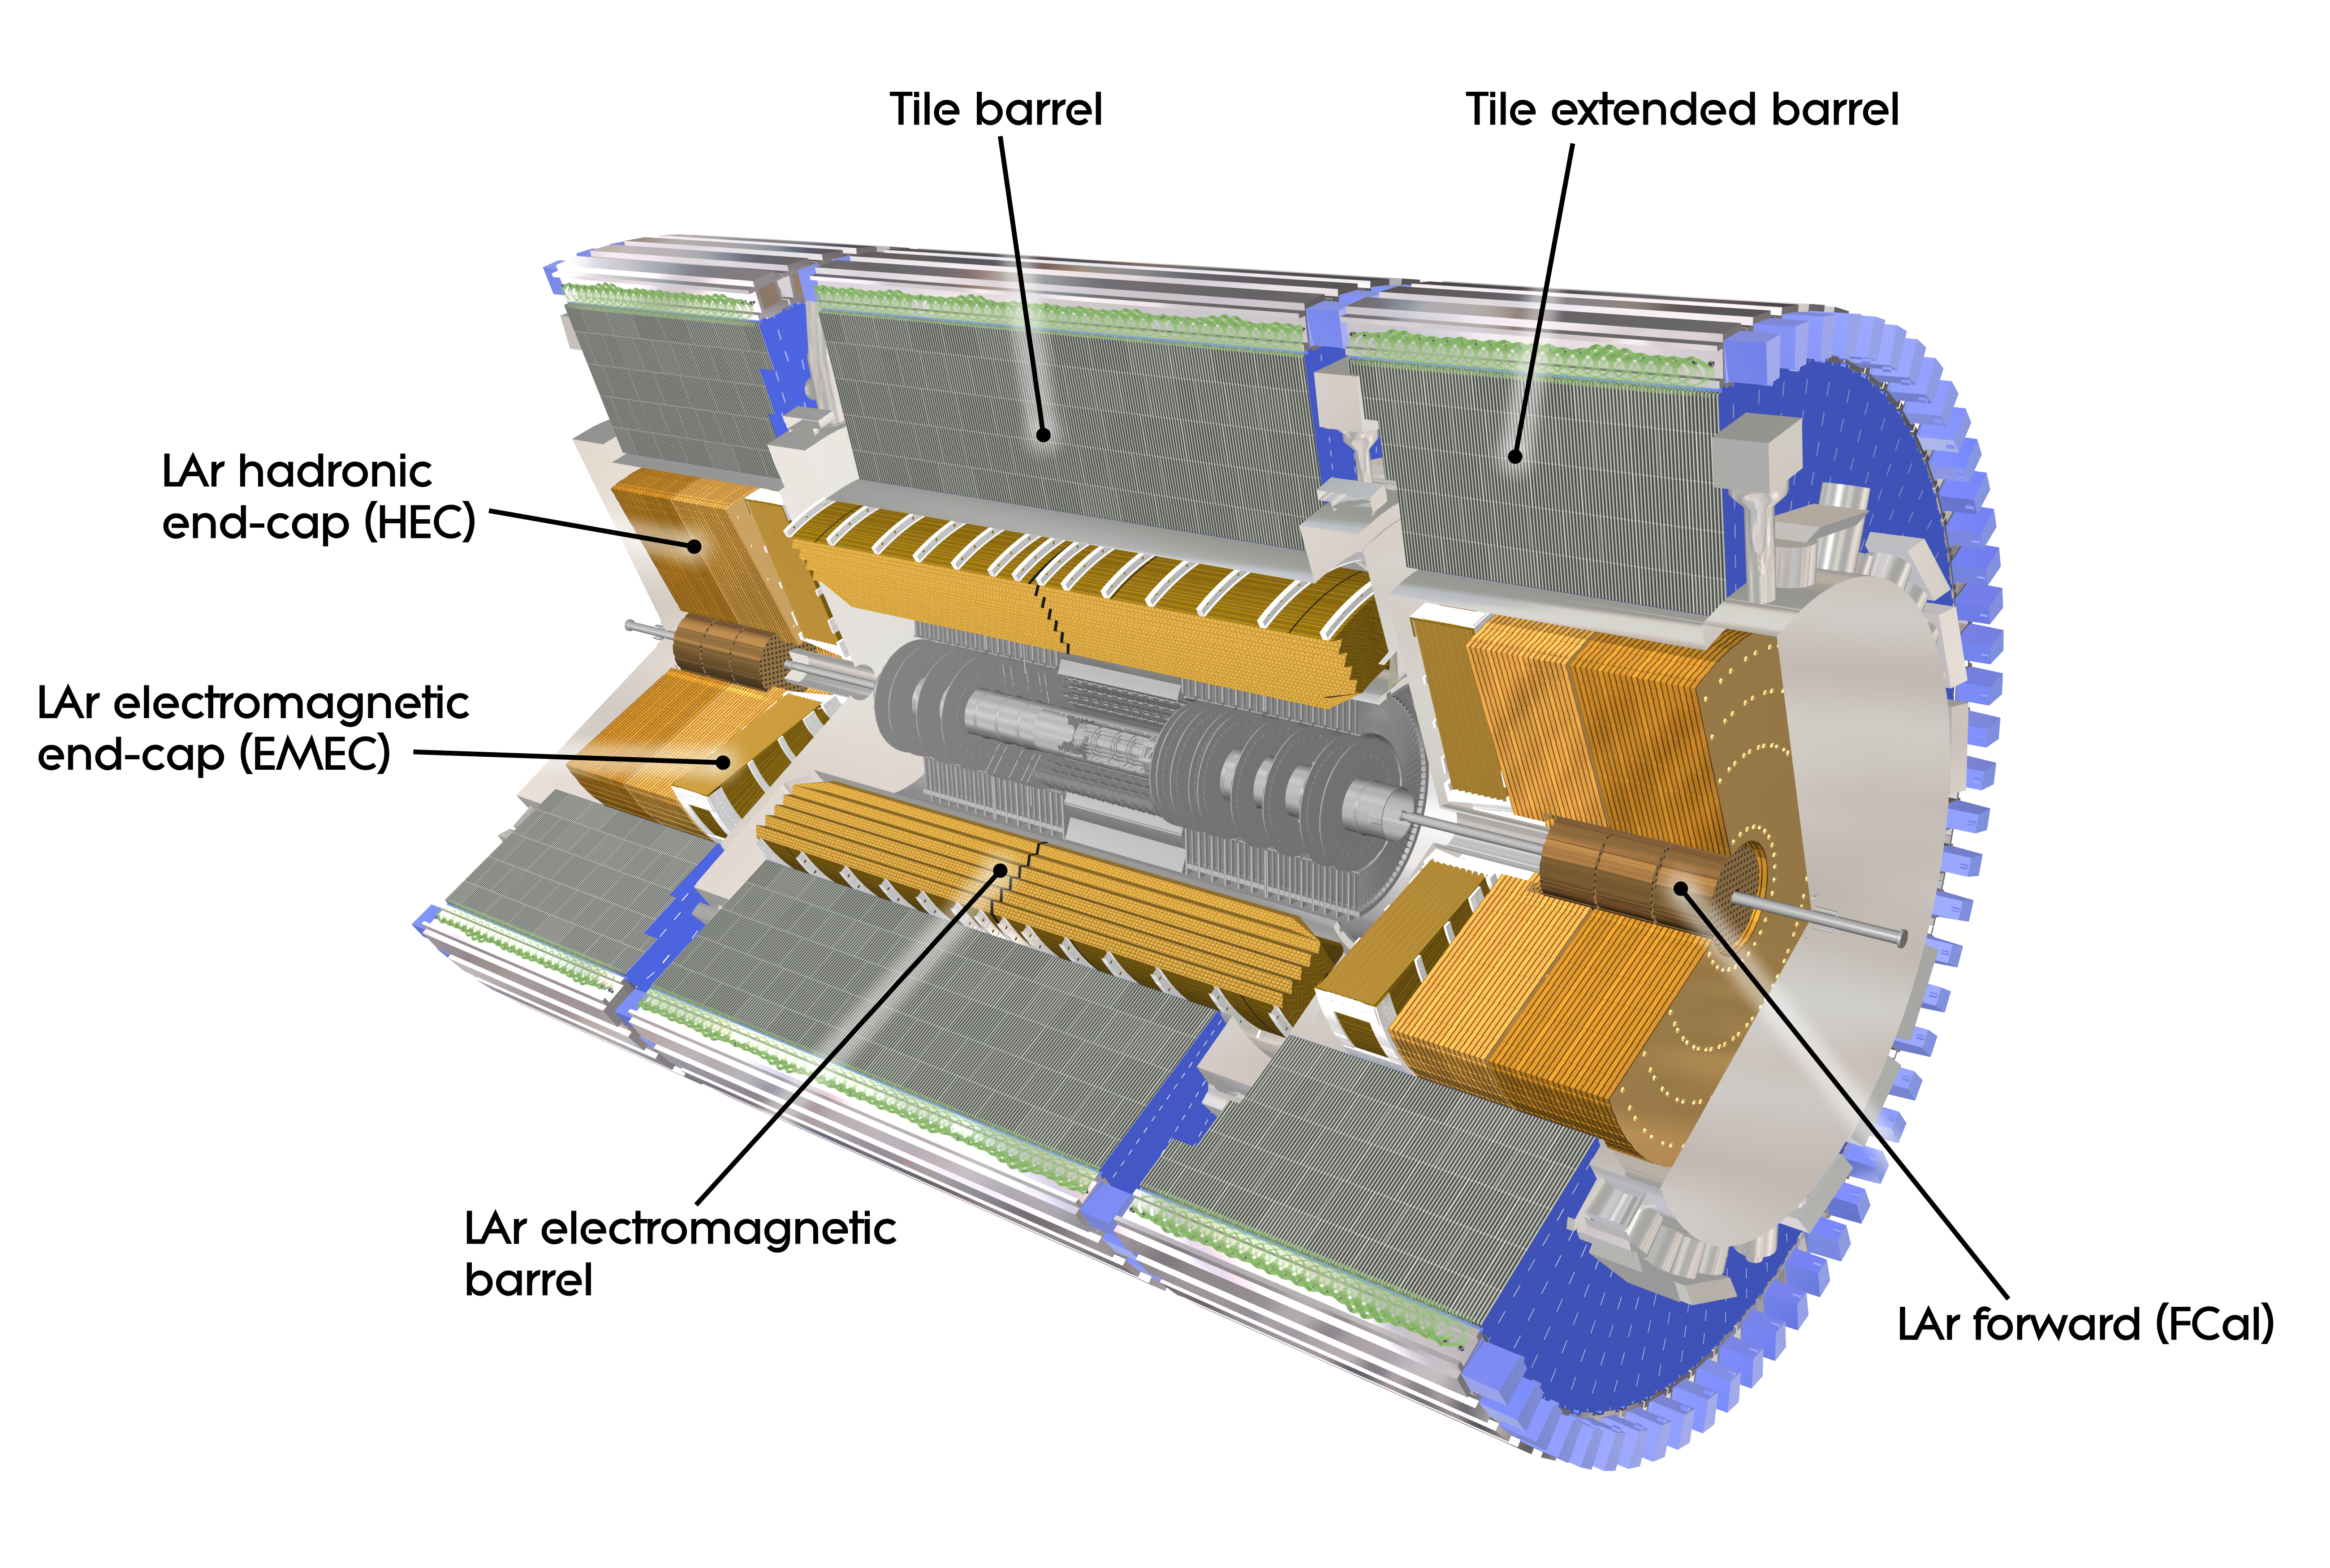
\includegraphics[width=0.7\textwidth]{figures/ch3/calorimeter.png}
	\caption{ATLAS calorimetery system \cite{calorimeter_img}}
	\label{fig:calorimeters}
\end{figure}

\subsection{Liquid Argon Calorimeter}
%regions
The LAr calorimeter is a sampling calorimeter designed to trigger on and measure the energies of electromagnetic particles, as well as hadronic particles in the high $\eta$ regions. It is divided in several regions, as shown in Figure \ref{fig:calorimeters}. For the region $|\eta| < 1.4$, the electromagnetic barrel (EMB) is responsible for electronic calorimetery, and provides high resolution energy, timing, and position measurements for electrons and photons passing through the detector. The electromagnetic endcap (EMEC) provides additional EM calorimetery up to $|\eta|<3.2$. In the region $1.4 < |\eta| < 3.2$, the hadronic endcap (HEC) provides hadronic calorimetery. For hadronic calorimetery In the region $|eta| < 1.4$, corresponding to a detector radii > 2.2m, the less expensive tile calorimeter (discussed in the next section) is used instead. A forward calorimeter (FCAL) extends the hadronic calorimetery coverage up to $3.1 < |\eta| = 4.8$ \cite{lar_tdr}. \\
 
 %construction
The LAr calorimeter is composed of liquid argon sandwiched between layers of absorber material and electrodes. Liquid argon is advantageous as a calorimeter active medium due to its natural abundance and low cost, chemical stability, radiation tolerance, and linear response over a large energy range \cite{lar_ssc}. The calorimeter is cooled to 87k by three cryostats: one barrel cryostat encompassing the EMB, and two endcap cryostats. The barrel cryostat also encloses the solenoid which produces the 2T magnetic field for the inner detector. Front end electronics are housed outside the cryostats and are used to process, store and transfer the calorimeter signals. \\ 

\subsubsection{Electromagnetic Calorimeter}
%accordion
For the electromagnetic calorimeters, the layers of electrodes and absorber materials are arranged in an an accordion shape, as illustrated in Figure \ref{fig:lar_accordion}. The accordion shape ensures that each half barrel is continuous in the azimuthal angle, which is a key feature for ensuring consistent high resolution measurements. Liquid argon permeates the space between the lead absorber plates, and a multilayer copper-polymide readout board runs through the center of the liquid argon filled gap. \\

\begin{figure}
        \centering
	\includegraphics[width=0.6\textwidth]{figures/ch3/lar_accordion.png}
	\caption{Diagram of a segment of the EMB, demonstrating the accordion plate arrangement \cite{lar_tdr}}
	\label{fig:lar_accordion}
\end{figure}

% detection 
The detection principle for the LAr calorimeter is the current created by electrons which are released when a charged particle ionizes the liquid argon. In the barrel region, the electrons are driven towards the center electrodes by a 2000V potential with a drift time of less than 450ns \cite{lar_overview}. In the endcaps the voltage varies as a function of the radius in order to maintain a flat response \cite{lar_tdr}. The amount of current produced by the ionized electrons is proportional to the energy of the particle creating the signal. Figure \ref{lar_pulse} shows the shape of the signal produced in the LAr calorimeter, before and after it undergoes shaping during the readout process. The shaping of the pulse enforces a positive peak and a negative tail, which ensures that subsequence pulses can be separated with the precision required for the 25ns LHC bunch spacing \cite{lar_tdr}. \\

\begin{figure}
        \centering
	\includegraphics[width=0.5\textwidth]{figures/ch3/lar_pulse.png}
	\caption{A LAr pulse as produced in the detector (triangle) and after shaping (curve) \cite{lar_tdr}}
	\label{fig:lar_pulse}
\end{figure}

\subsubsection{Hadronic End-cap Calorimeter}
The HEC sits radially beyond the EMEC. The copper absorber plates in the HEC are oriented perpendicular to the beamline, with LAr as the active medium. Each end-cap is divided into two independent wheels; the inner wheel uses 25mm copper plates, while the outer wheel uses 50mm plates as a cost saving measure. In each wheel, the 8.5mm plate gap is crossed by three parallel electrodes, creating and effective drift distance of 1.8mm. This gap is illustrated in Figure \ref{fig:hec}. Each wheel is divided into 32 wedge-shaped modules, each containing their own set of readout electronics.

\begin{figure}
        \centering
	\includegraphics[width=0.5\textwidth]{figures/ch3/hec.png}
	\caption{Readout gap structure in HEC \cite{lar_tdr}}
	\label{fig:hec}
\end{figure}

\subsubsection{Forward Calorimeter}
The forward range is covered by the FCAL, which provides both electromagnetic and hadronic calorimetry. It is composed of three active cylindrical modules; one EM module with copper absorber plates, and two hadronic modules with tungsten absorber plates. The plates are oriented perpendicular to the beamline, and LAr is used as the active material throughout.

\subsection{Tile Calorimeter}
The tile calorimeter (TileCal) provides hadronic calorimetry in the region $\eta < 1.7$, and surrounds the LAr calorimeter. It is responsible for measurements of jet energy and jet substructure, and also plays an important role in electron isolation and triggering (including muons) \cite{tile_tdr}. TileCal is composed of 3 sections, as shown in figure \ref{fig:calorimeters}; a barrel calorimeter sits directly outside the LAr EMB and provides coverage up to $\eta < 1.0$. Two extended barrel sections sit outside the LAr endcaps and cover the region $0.8 < \eta < 1.7$. \\

TileCal is a sampling calorimeter composed of steel and plastic scintillator plates as illustrated in Figure \ref{fig:tileCal}. A total of 460,000 scintillators are read out by wavelength-shifting fibers. The fibers are gathered to define cells and in turn read out by photomultiplier tubes, which amplify the signal and convert it to an electrical signature. Each cell has an approximate granularity of $\Delta\eta \times \Delta\phi = 0.1 \times 0.1$. Each barrel is divided azimuthally into 64 independent modules, an example of which is show in Figure \ref{fig:tileCal}. The modules are each serviced by front-end electronic housed in a water-cooled drawer on the exterior of the module. \\

\begin{figure}
        \centering
	\includegraphics[width=0.5\textwidth]{figures/ch3/tileWedge.png}
	\caption{TileCal wedge module \cite{tile_tdr} }
	\label{fig:tileCal}
\end{figure}

The detection principle of the TileCal is the production of light from hadronic particles interacting with the scintillating tiles. When a hadronic particle hits the steel plate, a shower of particles are produced. The interaction of the shower with the plastic scintillator produces photons, the number and intensity of which are proportional to the original particle's energy. \\


